\documentclass[12pt,a4]{article}
% \usepackage{draftwatermark}
\usepackage{background}
\usepackage{color}   %May be necessary if you want to color links
\usepackage{hyperref}
\hypersetup{
    colorlinks=true, %set true if you want colored links
    linktoc=all,     %set to all if you want both sections and subsections linked
    linkcolor=blue,  %choose some color if you want links to stand out
}
\textwidth 170 mm
\oddsidemargin -8 mm
\evensidemargin -8 mm
%\SetWatermarkScale{3.0}
\SetBgColor{red}
\SetBgOpacity{0.1}
\SetBgScale{10}
%\SetBgContents{\hspace{9mm}DRAFT \hspace{0mm}\vspace{2mm} \includegraphics[width=5mm]{Alfresco_logo_CMYK_white}} 

\begin{document}
\begin{center}
{\Large How to make an alfresco server join a Windows Domain}

\vspace{5mm}

\Large{To achieve better kerberos security}

\vspace{5mm}
{\bf Alex Madon}
\vspace{5mm}

\today

\vspace{15mm}
{\huge To be reviewed}

\end{center}
\vspace{5mm}

\newpage

\tableofcontents

\newpage

\section{Introduction}
In ticket 62987 the customer informs us that Microsoft document at URL:
\begin{verbatim}
http://technet.microsoft.com/en-us/library/cc738673%28v=ws.10%29.aspx
\end{verbatim}
mentions that the option:

``Trust this user for delegation to any service (Kerberos only)''
	
is

``Not recommended. This enables unconstrained delegation.''


In our current official documentation we say to tick that option for the alfrescohttp user.

A better option would be to use the other option:

``Trust this user for delegation to specified services only''
	

    ``Use Kerberos only'': Enables constrained delegation without protocol transition.

My test setup is as follow:
\begin{itemize}
\item a linux debian server madona.example.foo with IP 10.69.69.1 that runs alfresco kerberos with realm EXAMPLE.FOO 
\item a Active Directory 2003 win2003.example.foo with IP 10.69.69.99 that is a controller for domain EXAMPLE.FOO
\item (optionally) a XP workstation winxp.example.foo

\end{itemize}

The goal is to be able to enable delegation for this account only when it comes from madona.example.foo
However, the server named MADONA does not appear in the Directory computer list.
The goal of this paper is to describe the simplest way to make that computer appear. In Microsoft terminology, the linux server MADONA needs to {\bf join the domain} EXAMPLE.FOO.

\begin{figure}[h]
 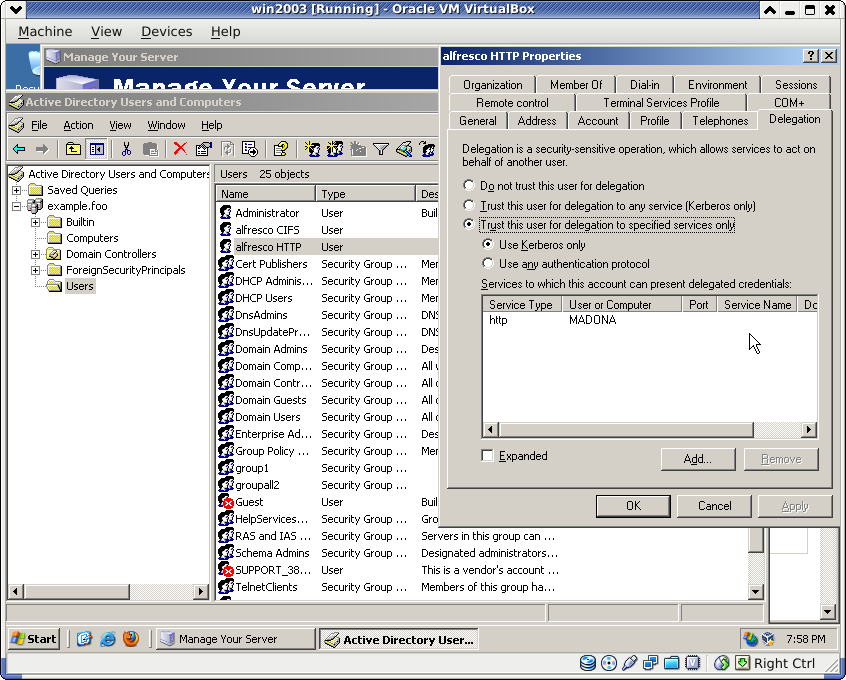
\includegraphics[width=120mm]{goal}
\caption{Our goal: the delegation is subject to the constraint that the request needs to come from MADONA on HTTP. This picture has been taken AFTER having added the MADONA server using the method described in this article. Before the addition, you simple cannot see the MADONA server as a select-able computer.}
\end{figure}

\section{What does joining a domain mean?}
To understand what joining a domain means, we can use a sample Windows XP client and tell it to join the EXAMPLE.FOO domain.
To reverse engineer the meaning of this action, sniffing the network traffic between the XP client and Active Directory is helpful.
We can sniff the ldap traffic port 389. the kerberos traffic port 88, and the smb traffic ports 137, 138, 139, 445.

From a User Interface point of view, in XP, this means go to computer -> Properties -> join a domain.

You are then asked to authentication as an Active Directory administrator.

The analysis of the network dumps shows that the XP client authenticates using kerberos the the AD server and then creates a WINXP\$ folder using smb port 445 and then add three attributes in the directory for the DN

\begin{verbatim}
dn: CN=WINXP,CN=Computers,DC=example,DC=foo
\end{verbatim}

the three attributes being:

\begin{verbatim}
dNSHostName: winxp.example.foo
servicePrincipalName: HOST/WINXP
servicePrincipalName: HOST/winxp.example.foo
\end{verbatim}

\section{How to make a Linux server join a domain?}
The internet mentions several tools to make a linux computer join a Windows domain see for instance
https://help.ubuntu.com/community/ActiveDirectoryWinbindHowto
where some solutions are listed:
\begin{itemize}
\item samba windbind
\item Centrify Express
\item Likewise Open domainjoin-cli
\end{itemize}
However, those solutions seems to be very involved. Another page on the web 

\begin{verbatim}
http://pig.made-it.com/pig-adusers.html
Creating Active Directory Accounts
Using LDIF files and OpenLDAP tools
© 2009 Dennis Leeuw
\end{verbatim}
confirms the hopes we had at looking at the network dump that a solution based only on LDAP (and maybe SMB) is possible.

\section{Make linux ldap clients able to write to Active Directory}
Assuming that your linux server has the /etc/krb5.conf below:

\begin{verbatim}
[libdefaults]
default_realm = EXAMPLE.FOO
default_tkt_enctypes = rc4-hmac
default_tgs_enctypes = rc4-hmac
permitted_enctypes= rc4-hmac
forwardable = true

[realms]
EXAMPLE.FOO = {
  kdc = 10.69.69.99
  admin_server = 10.69.69.99
 }
[domain_realm]
	.example.foo = EXAMPLE.FOO
\end{verbatim}
then you can authenticate using kerberos kinit command 'administrator' to AD:

\begin{verbatim}
kinit administrator
\end{verbatim}

Then you can test using ldapsearch if you are able to use kerberos GSSAPI to communicate with AD:
\begin{verbatim}
ldapsearch -Y GSSAPI \
-h win2003.example.foo \
-U administrator \
-b "DC=example,DC=foo" "(cn=WINXP)"
\end{verbatim}

I encountered two issues:

\subsection{Missing gssapi library}
\begin{verbatim}
madon@madona:~$ ldapsearch -v -Y GSS-SPNEGO \
-h 10.69.69.99 -U administrator \
-b "DC=example,DC=foo" "(sAMAccountName=user1)"
ldap_initialize( ldap://10.69.69.99 )
ldap_sasl_interactive_bind_s: Unknown authentication method (-6)
	additional info: SASL(-4): no mechanism available: No worthy mechs found
\end{verbatim}

This was resolved by installing the package:

\begin{verbatim}
libsasl2-modules-gssapi-mit
\end{verbatim}
\subsection{Wrong DNS entry}

\begin{verbatim}
madon@madona:~$ ldapsearch -Y GSSAPI -h 10.69.69.99 \
-U administrator \
-b "DC=example,DC=foo" "(sAMAccountName=user1)"
SASL/GSSAPI authentication started
ldap_sasl_interactive_bind_s: Local error (-2)
	additional info: SASL(-1): generic failure: GSSAPI Error: Unspecified GSS failure.  Minor code may provide more information (Server not found in Kerberos database)
\end{verbatim}

This was resolved by appending to the /etc/hosts of the linux server:

\begin{verbatim}
10.69.69.99 win2003.example.foo 
\end{verbatim}


\section{Creating the record for the linux server in AD}

To actually make the MADONA server ``join'' the network, we now just need to write one LDIF file ``new.ldif'' that contains:
\begin{verbatim}
dn: CN=MADONA,CN=Computers,DC=example,DC=foo
changetype: add
objectClass: top
objectClass: person
objectClass: organizationalPerson
objectClass: user
objectClass: computer
cn: MADONA
distinguishedName: CN=MADONA,CN=Computers,DC=example,DC=foo
objectCategory: CN=Computer,CN=Schema,CN=Configuration,dc=example,dc=foo
instanceType: 4
displayName: MADONA$
name: MADONA
userAccountControl: 4096
codePage: 0
countryCode: 0
accountExpires: 0
sAMAccountName: MADONA$
dNSHostName: MADONA.example.foo
servicePrincipalName: HOST/MADONA
servicePrincipalName: HOST/MADONA.example.foo
\end{verbatim}
and then insert it with the openldap ``ldapmodify'' client:
\begin{verbatim}
ldapmodify -Y GSSAPI -h win2003.example.foo -U administrator -f new.ldif
\end{verbatim}

You can check that now the computer MADONA appears in the list of computers in AD.
A posteriori we notice that no SMB commands were necessary, we created the record with just one single LDAP add request.


\section{Confirming and testing}
We are now able to set the more restrictive delegation: the one showed in the above picture.
Testing access to Share confirms that this delegation is enough to make alfresco Share work.

\end{document}
